\chapter{Process for Generating EnAcT Inputs}

EnAcT requires the distributions for each encounter property to be able to generate millions of encounters that fall into these distributions. To generate these distributions that are realistic to what can be seen in the NAS, the Modeling and Simulation Branch developed a process to determine these distributions. A software tool that the branch developed, called the Trajectory Conflict Probe \cite{paglione:2008}, is the first step of the process. It inputs recorded flight plans and surveillance position reports and predicts when two aircraft are on a path that could violate these separation distances. Air traffic controllers issue clearances to alter one or both aircraft’s paths to resolve these conflicts before they occur. The tool records both the initial event and when the conflict is resolved. This allows the team to determine theoretical encounters from recorded air traffic data that had no actual encounters occurring due to air traffic controller intervention. \ref{fig:tcp} shows the flow of the Trajectory Conflict Probe program. 

\begin{figure}
\centering
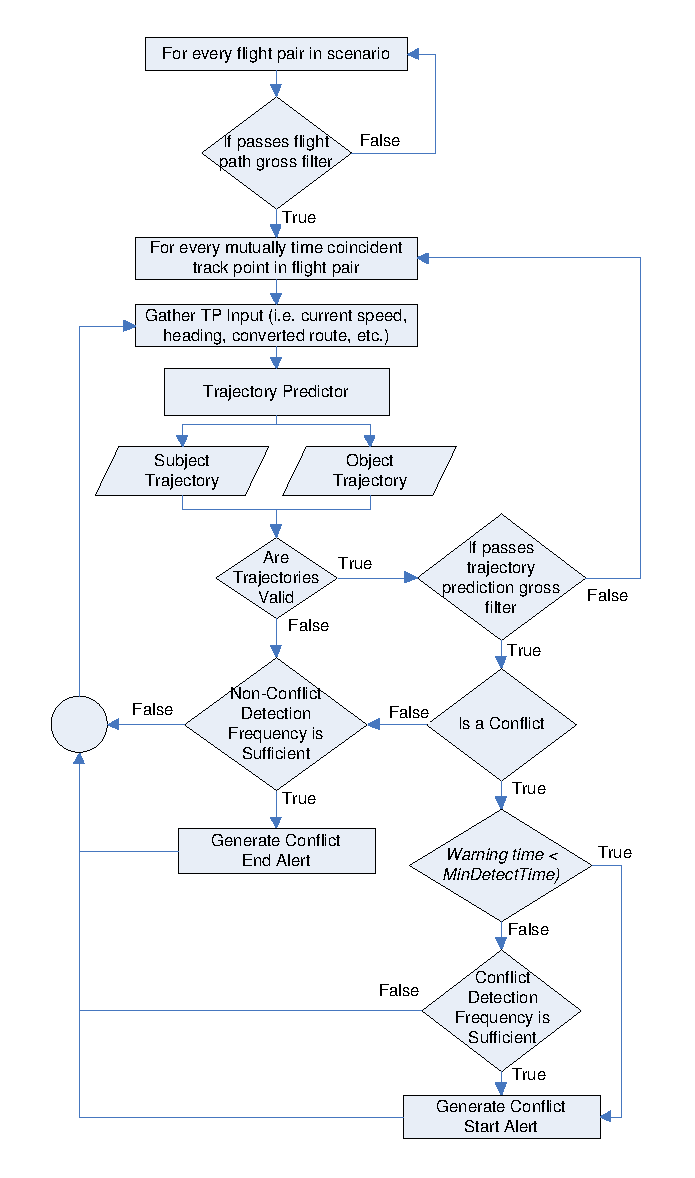
\includegraphics[scale=0.95]{Figures/TrajectoryConflictProbeFlowChart.pdf}
\caption{Flowchart of the Trajectory Conflict Probe Algorithm}
\floatfoot{\textit{Note.} This program analyzes each flight pair that has paths that are close enough to potentially cause a conflict \cite{paglione:2008}. Using a trajectory engine and the relevant clearance information, this program can predict where a conflict could have occurred if it were not for controller intervention, as long as the generated trajectories are valid.}
\label{fig:tcp}
\end{figure}

As \ref{fig:tcp} illustrates, the Trajectory Conflict Probe performs a pairwise analysis of flights from a given air traffic scenario. It considers each aircraft's flight plans, amendments, issued controller clearances, and surveillance position reports. The software first runs a gross filter to check rapidly for approximate temporal and spatial overlap of the pair of aircraft, based on the given position reports, or track data, of the two aircraft. This filter removes flight pairs that have no potential spatial overlap, cutting down the processing needed. If the pair passes this initial gross filter, the tool is called the Trajectory Predictor, which generates a predicted trajectory at each incremental time step that both aircraft have available track data. These predicted trajectories pass through a sequence of filters to determine if any predicted conflicts (violations of separation standards) or encounters (larger separation events) occur. 

Once an encounter is detected, the algorithm checks to see if the encounter occurs within the user defined predicted warning time. If it does, it immediately records the encounter. If the detected encounter is predicted to occur outside of the warning time, the algorithm checks the conflict detection frequency. The encounter detection frequency is the number of times the conflict probe predicts the encounter for each track instantiated trajectory before the predicted event. The user defines a percentage of the track instantiated trajectories that have a positive detection of the predicted event for it to be recorded as an encounter. The program continues to track the prediction event for each track instantiated trajectory. Once the program detects the encounter has ended, it starts to count these events from each new trajectory. If this percentage is met, the encounter has ended, and the results are recorded. These checks are the frequency checks referenced in \ref{fig:tcp} flowchart and act as stability filters for the encounter predictions. The program outputs the resulting encounters it detects as alert messages. These alert messages include the time of detection, the location of the predicted event, and the location of the aircraft when the event was predicted.

Using the Trajectory Conflict Probe tool, the characteristics of potential NAS conflicts and encounters can be estimated and matched by the encounter generation algorithm. The encounter properties that were considered in this study are: Encounter/Conflict Location, Horizontal Separation Distance, Vertical Separation Distance, Encounter Angle, Aircraft Type, and Vertical Phase of Flight.

\section{Encounter Properties}
Aircraft must be safely separated horizontally and vertically as they fly in the NAS. Different airspace has slightly different separation minima. Air traffic controllers manage the aircraft in Class A airspace to ensure safe separation at or beyond the required distances. The Modeling and Simulation Branch has developed a software tool, called the Trajectory Conflict Probe \cite{paglione:2008}, that inputs recorded flight plans and surveillance position reports and predicts when two aircraft are on a path that could violate these separation distances. Air traffic controllers issue clearances to alter one or both aircraft’s paths to resolve these conflicts before they occur. The tool records both the initial event and when the conflict is resolved. 

As \ref{fig:tcp} illustrates, the Trajectory Conflict Probe performs a pairwise analysis of flights from a given air traffic scenario. It considers each aircraft’s flight plans, amendments, issued controller clearances, and surveillance reports. The software first runs a gross, or coarse, filter to check rapidly for approximate temporal and spatial overlap of the pair of aircraft. This filter removes flight pairs that have no potential spatial overlap, cutting down the processing needed. If the pair passes this initial gross filter, the tool is called the Trajectory Predictor, which generates a predicted trajectory at each incremental time step that both aircraft have available track data. These predicted trajectories pass through a sequence of filters to determine if any predicted conflicts (violations of separation standards) or encounters (larger separation events) occur. The algorithm requires a user specified number of multiple positive detections within a specified number of times increments to determine whether the event is an encounter or conflict. Similarly, once detection and posting of the encounter or conflict occurs, it takes several negative detections to end the event’s posting. These checks are the frequency checks referenced in the \ref{fig:tcp} flowchart and act as stability filters for the encounter/conflict predictions. Therefore, the Trajectory Conflict Probe application provides a list of predicted conflicts and encounters for estimating the input encounter properties required by EnAcT.

The focus of this study is to document the encounter properties produced by the Trajectory Conflict Probe of the initial predicted event or first posting of the predicted encounter. There are many characteristics that can be studied; several of these were the subject of previous work performed in \cite{paglione:2008}. This study focuses on six encounter properties considered important for input into the conflict generator application as discussed in \hyperref[chap:enactprogram]{Chapter 3 EnAcT Program}.

\subsection{Horizontal Separation}
Horizontal separation is the minimum horizontal distance between two aircraft (ownship and intruder) during an encounter event, measured in nautical miles (NM). Predicted events are counted and grouped into 1 NM bins, from 0 to 5 NM.

\subsection{Vertical Separation}
Vertical separation is the minimum difference in altitude between two aircraft during an encounter event, measured in feet (ft.). Predicted events are counted and grouped into 500 ft. bins, from 0 to 2000 ft.

\subsection{Encounter Angle}
Encounter angle is the difference between the aircraft headings at the closest point of approach, measured in degrees (\textdegree). Predicted events are counted and grouped into four bins: 0\textdegree to 15\textdegree, 15\textdegree to 90\textdegree, 90\textdegree to 165\textdegree, and 165\textdegree to 180\textdegree. 

The first bin, 0\textdegree to 15\textdegree, represents a predicted encounter where the two aircraft are either in-trail (following the same horizontal path) or are on similar paths and closing at a very shallow angle. A special case of these events, referred to as overtake, is when the aircraft are on the same path and the trailing aircraft is faster than the leading aircraft.

The second and third bins, 15\textdegree to 90\textdegree and 90\textdegree to 165\textdegree, represent predicted conflicts that have aircraft crossing paths from the right or left. The last bin from 165\textdegree to 180\textdegree represents predicted conflict events from aircraft trajectories that are approaching one another either head-on or near head-on.

These different categories of encounter angles are likely to present different challenges to systems that need to predict and resolve them. For example, in-trail encounter angles are particularly sensitive to errors in aircraft speed calculations, while head-on events may have high closure rates requiring quick application of conflict resolutions.

\subsection{Aircraft Type}
The aircraft type parameter is a two- to four-character ICAO aircraft type designator representing the type of aircraft involved in the encounter event. Each aircraft has its own code. For example, Boeing 737-700 aircraft have ICAO code B737, and Airbus A321 aircraft have ICAO code A321. The choice of aircraft type naturally affects the nominal aircraft performance data retrieved from BADA, such as speed profile, climb and descent rates, and weight. This aircraft performance information allows the encounter generator program to generate customized trajectories for the aircraft involved in an encounter.

\subsection{Encounter Location}
The encounter location is defined by the latitude, longitude, and altitude of the subject aircraft of the predicted conflict event. Location is measured in decimal degrees (\textdegree) for both latitude and longitude, and in feet (ft.) for altitude. \ref{fig:map} displays the horizontal location of predicted encounter events during the study documented in \cite{paglione:2008}.

\begin{figure}[H]
\centering
\includegraphics{Figures/EncounterMap.png}
\caption{Overlay of Accumulated Encounters/Conflicts Across the NAS \cite{paglione:2008}}
\label{fig:map}
\end{figure}
~\\

The symbol and color used to denote each predicted encounter event represents the altitude at which the predicted event occurs. EnAcT uses this information to create conflicts that occur in locations that are like those that have been presumably resolved by air traffic controllers in the NAS.

\subsection{Vertical Phase of Flight}
The vertical phase of flight describes whether the aircraft is climbing, descending, or level. An aircraft is ascending (ASC) when it is increasing in altitude and descending (DEC) when it is decreasing in altitude. An aircraft is level (LEV) when the aircraft remains at a constant altitude. These metrics capture information regarding the vertical profiles of the flights during the predicted encounter event.

In this study, the vertical phase of flight for both aircraft is considered, creating a vertical phase of flight pair. There are nine combinations of vertical phases of flight. \ref{table:vpof} presents these combinations. The first code before the underscore denotes the vertical phase of flight of the ownship, while the code after the underscore denotes the vertical phase of flight of the intruder.

\begin{table}[H]
\caption{Vertical Phase of Flight Pair Codes}
\label{table:vpof}
\begin{center}
\begin{tabular}{|c|} 
    \hline
    \textbf{PAIR CODES} \\
    \hline
    ASC\_ASC \\
    \hline
    ASC\_DSC \\
    \hline
    ASC\_LEV \\
    \hline
    DSC\_ASC \\
    \hline
    DSC\_DSC \\
    \hline
    DSC\_LEV \\
    \hline
    LEV\_ASC \\
    \hline
    LEV\_DSC \\
    \hline
    LEV\_LEV \\
    \hline
\end{tabular}
\end{center}
\end{table}
~\\

\subsection{Horizontal Phase of Flight}
Horizontal phase of flight describes whether the aircraft is turning left, turning right, or going straight ahead at the closest point of approach. This parameter is not considered for this study and is not used in EnAcT currently. It may be revisited in the future but is included here simply for reference.